% Options for packages loaded elsewhere
\PassOptionsToPackage{unicode}{hyperref}
\PassOptionsToPackage{hyphens}{url}
\PassOptionsToPackage{dvipsnames,svgnames,x11names}{xcolor}
%
\documentclass[
  letterpaper,
  DIV=11,
  numbers=noendperiod]{scrartcl}

\usepackage{amsmath,amssymb}
\usepackage{iftex}
\ifPDFTeX
  \usepackage[T1]{fontenc}
  \usepackage[utf8]{inputenc}
  \usepackage{textcomp} % provide euro and other symbols
\else % if luatex or xetex
  \usepackage{unicode-math}
  \defaultfontfeatures{Scale=MatchLowercase}
  \defaultfontfeatures[\rmfamily]{Ligatures=TeX,Scale=1}
\fi
\usepackage{lmodern}
\ifPDFTeX\else  
    % xetex/luatex font selection
\fi
% Use upquote if available, for straight quotes in verbatim environments
\IfFileExists{upquote.sty}{\usepackage{upquote}}{}
\IfFileExists{microtype.sty}{% use microtype if available
  \usepackage[]{microtype}
  \UseMicrotypeSet[protrusion]{basicmath} % disable protrusion for tt fonts
}{}
\makeatletter
\@ifundefined{KOMAClassName}{% if non-KOMA class
  \IfFileExists{parskip.sty}{%
    \usepackage{parskip}
  }{% else
    \setlength{\parindent}{0pt}
    \setlength{\parskip}{6pt plus 2pt minus 1pt}}
}{% if KOMA class
  \KOMAoptions{parskip=half}}
\makeatother
\usepackage{xcolor}
\setlength{\emergencystretch}{3em} % prevent overfull lines
\setcounter{secnumdepth}{-\maxdimen} % remove section numbering
% Make \paragraph and \subparagraph free-standing
\makeatletter
\ifx\paragraph\undefined\else
  \let\oldparagraph\paragraph
  \renewcommand{\paragraph}{
    \@ifstar
      \xxxParagraphStar
      \xxxParagraphNoStar
  }
  \newcommand{\xxxParagraphStar}[1]{\oldparagraph*{#1}\mbox{}}
  \newcommand{\xxxParagraphNoStar}[1]{\oldparagraph{#1}\mbox{}}
\fi
\ifx\subparagraph\undefined\else
  \let\oldsubparagraph\subparagraph
  \renewcommand{\subparagraph}{
    \@ifstar
      \xxxSubParagraphStar
      \xxxSubParagraphNoStar
  }
  \newcommand{\xxxSubParagraphStar}[1]{\oldsubparagraph*{#1}\mbox{}}
  \newcommand{\xxxSubParagraphNoStar}[1]{\oldsubparagraph{#1}\mbox{}}
\fi
\makeatother


\providecommand{\tightlist}{%
  \setlength{\itemsep}{0pt}\setlength{\parskip}{0pt}}\usepackage{longtable,booktabs,array}
\usepackage{calc} % for calculating minipage widths
% Correct order of tables after \paragraph or \subparagraph
\usepackage{etoolbox}
\makeatletter
\patchcmd\longtable{\par}{\if@noskipsec\mbox{}\fi\par}{}{}
\makeatother
% Allow footnotes in longtable head/foot
\IfFileExists{footnotehyper.sty}{\usepackage{footnotehyper}}{\usepackage{footnote}}
\makesavenoteenv{longtable}
\usepackage{graphicx}
\makeatletter
\newsavebox\pandoc@box
\newcommand*\pandocbounded[1]{% scales image to fit in text height/width
  \sbox\pandoc@box{#1}%
  \Gscale@div\@tempa{\textheight}{\dimexpr\ht\pandoc@box+\dp\pandoc@box\relax}%
  \Gscale@div\@tempb{\linewidth}{\wd\pandoc@box}%
  \ifdim\@tempb\p@<\@tempa\p@\let\@tempa\@tempb\fi% select the smaller of both
  \ifdim\@tempa\p@<\p@\scalebox{\@tempa}{\usebox\pandoc@box}%
  \else\usebox{\pandoc@box}%
  \fi%
}
% Set default figure placement to htbp
\def\fps@figure{htbp}
\makeatother

\usepackage{booktabs}
\usepackage{caption}
\usepackage{longtable}
\usepackage{colortbl}
\usepackage{array}
\usepackage{anyfontsize}
\usepackage{multirow}
\KOMAoption{captions}{tableheading}
\makeatletter
\@ifpackageloaded{caption}{}{\usepackage{caption}}
\AtBeginDocument{%
\ifdefined\contentsname
  \renewcommand*\contentsname{Table of contents}
\else
  \newcommand\contentsname{Table of contents}
\fi
\ifdefined\listfigurename
  \renewcommand*\listfigurename{List of Figures}
\else
  \newcommand\listfigurename{List of Figures}
\fi
\ifdefined\listtablename
  \renewcommand*\listtablename{List of Tables}
\else
  \newcommand\listtablename{List of Tables}
\fi
\ifdefined\figurename
  \renewcommand*\figurename{Figure}
\else
  \newcommand\figurename{Figure}
\fi
\ifdefined\tablename
  \renewcommand*\tablename{Table}
\else
  \newcommand\tablename{Table}
\fi
}
\@ifpackageloaded{float}{}{\usepackage{float}}
\floatstyle{ruled}
\@ifundefined{c@chapter}{\newfloat{codelisting}{h}{lop}}{\newfloat{codelisting}{h}{lop}[chapter]}
\floatname{codelisting}{Listing}
\newcommand*\listoflistings{\listof{codelisting}{List of Listings}}
\makeatother
\makeatletter
\makeatother
\makeatletter
\@ifpackageloaded{caption}{}{\usepackage{caption}}
\@ifpackageloaded{subcaption}{}{\usepackage{subcaption}}
\makeatother

\usepackage{bookmark}

\IfFileExists{xurl.sty}{\usepackage{xurl}}{} % add URL line breaks if available
\urlstyle{same} % disable monospaced font for URLs
\hypersetup{
  pdftitle={Group3\_EDA\_ProjectPlan},
  pdfauthor={Daniel Rishea, Maria Granados, Mosaab Saleem},
  colorlinks=true,
  linkcolor={blue},
  filecolor={Maroon},
  citecolor={Blue},
  urlcolor={Blue},
  pdfcreator={LaTeX via pandoc}}


\title{Group3\_EDA\_ProjectPlan}
\author{Daniel Rishea, Maria Granados, Mosaab Saleem}
\date{}

\begin{document}
\maketitle


\section{Romantic Interest in Speed
Dating}\label{romantic-interest-in-speed-dating}

\subsection{Introduction}\label{introduction}

This project investigates the attributes that contribute to
\emph{romantic interest} in a speed dating context. The dataset,
obtained from OpenML (Speed Dating Dataset; OpenML ID 40536), contains
outcomes of speed dating events conducted between 2002 and 2004,
including lifestyle and demographic information about both participants.

Previous studies have used this dataset to predict ``matches'' between
participants (Fisman et al., 2006). However, we noted that the
experimental design favoured the subject of the date, which provided an
unequal number of features compared to their partner. Consequently, we
reframed our problem: instead of predicting matches, we aim to predict
the \textbf{partner's decision} (binary variable: \emph{decision} =
yes/no) regarding whether they would like to meet the subject again.

Specifically, we seek to:

\begin{enumerate}
\def\labelenumi{\arabic{enumi}.}
\tightlist
\item
  Examine the relationship between \textbf{self-reported subject
  attributes} (how individuals describe themselves) and \textbf{partner
  perceptions} (how those attributes are rated by the partner).
\item
  Compare how these factors differ across \textbf{gender}.
\item
  Identify which features most strongly predict \emph{romantic interest}
  in this context.
\end{enumerate}

\subsection{Exploratory Data Analysis}\label{exploratory-data-analysis}

We first completed data cleaning and exploratory data analysis (EDA).
This step was essential to ensure we could extract insights from the
dataset, to guide the choice of appropriate models and evaluation
metrics in line with our problem statement.

\subsubsection{Dataset Description}\label{dataset-description}

The original data contained 121 features and 8,378 observations.
However, 87.4\% of rows contained at least one missing value. The
original dataset presented several challenges:

\begin{itemize}
\item
  High number of missing values in some features.
\item
  High dimensionality with many overlapping features, resulting in high
  correlations between many features and target variable.
\item
  Unclear feature nomenclature. This was a considerable challenge, which
  required an iterative approach to cross-reference variables with
  documentation and related literature. Although time-intensive, this
  was essential to select meaningful features that aligned with our
  research question.
\end{itemize}

\subsubsection{Data Cleaning
Methodology}\label{data-cleaning-methodology}

To prepare the data for Exploratory Data Analysis (EDA), we completed
the following steps:

\begin{itemize}
\tightlist
\item
  Cross-referenced variables with documentation to keep only relevant
  variables:

  \begin{itemize}
  \tightlist
  \item
    Removed feature ranges when raw numeric values were already
    available.
  \item
    To avoid data leakage, features directly correlated with the target
    variable were removed (e.g., ``match,'' ``interest correlation'').
  \item
    Dropped irrelevant columns (e.g., ``expected,'' ``happy,''
    ``prob\_liked'').
  \end{itemize}
\item
  After filtering features, we removed rows with missing values in the
  remaining dataset. We took this approach to ensure we were retaining
  as many relevant observations as possible, as the original dataset had
  80\% missing observations.

  \begin{itemize}
  \tightlist
  \item
    Overall missing values for the relevant features were 57.7\%.
  \item
    When calculated by column, this was a considerable improvement, with
    the top three fields with missing values showing less than 15\%
    nulls present.
  \end{itemize}
\end{itemize}

\begin{table}
\fontsize{12.0pt}{14.4pt}\selectfont
\begin{tabular*}{\linewidth}{@{\extracolsep{\fill}}lrr}
\toprule
Feature & NullCount & NullPercent \\ 
\midrule\addlinespace[2.5pt]
shared\_interests\_o & 1076 & 12.84 \\ 
ambitous\_o & 722 & 8.62 \\ 
funny\_o & 360 & 4.30 \\ 
\bottomrule
\end{tabular*}
\end{table}

\begin{itemize}
\tightlist
\item
  Renamed target variable to \emph{decision} for clarity.
\item
  Out-of-range values (expected 1--10 scale) were handled using three
  strategies:

  \begin{enumerate}
  \def\labelenumi{\arabic{enumi}.}
  \tightlist
  \item
    Retained values as-is,
  \item
    Removed out-of-range values,
  \item
    Rescaled using min--max transformation.
  \end{enumerate}
\end{itemize}

For the EDA, we retained values as-is to assess their distribution and
impact before finalising an approach. Our final cleaned dataset included
\textbf{33 features and 6,949 observations} (see Appendix for details on
the final dataset).

\subsubsection{Target Variable Balance}\label{target-variable-balance}

The dataset is relatively balanced as shown below. As class imbalance is
not severe, the risk of class imbalance bias is low which supports the
use of accuracy as a baseline evaluation metric, but nuanced metrics
(F1, ROC-AUC) will still be important.

\pandocbounded{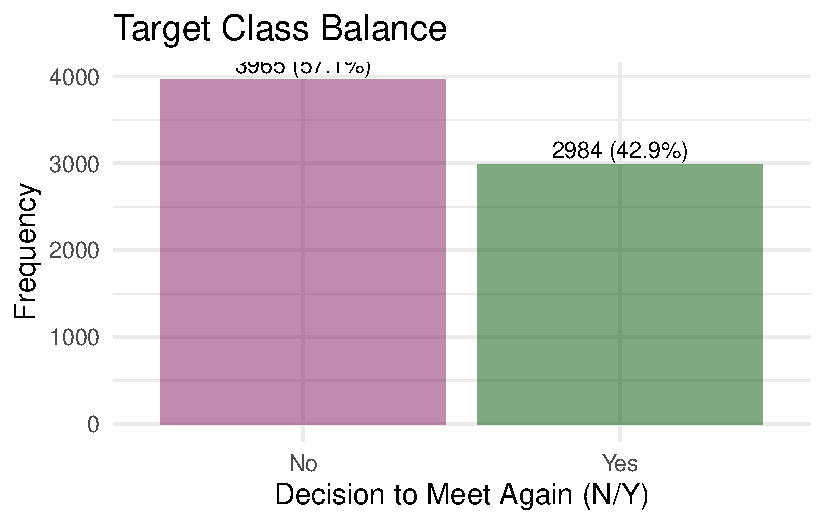
\includegraphics[keepaspectratio]{EDA-Plan_files/figure-pdf/features_balance-1.pdf}}

\subsubsection{Feature Distributions and
Trends}\label{feature-distributions-and-trends}

Key insights analysis show:

\begin{itemize}
\tightlist
\item
  \textbf{Gender and characteristics interaction:}

  \begin{itemize}
  \item
    \textbf{Subject self-assessed characteristics:} There is
    considerable overlap across most traits, with the exception of
    female partners seemingly favouring male subjects that self-report
    highly for attractiveness and intelligence, whilst male partners are
    seemingly less picky. It's interesting to point out that
    self-ratings by the subject do not seem to have a high effect on the
    final decision for male partner / female subject pairs, but yes for
    the female partners..
  \item
    \textbf{Subject's perceived characteristics}: The subject's
    perceived characteristics by the partner show stronger
    differentiation, with perceived attractiveness, funny, and shared
    interest providing a clear indication of a favourable decision.
    There are some gender differences, with intelligence being a weaker
    indicator for male partner / female subject pairs, whilst female
    partners seem to highly regard this trait in comparison to male
    partners.
  \item
    \textbf{Subject's interests}: The subject's interests also have
    considerable overlaps, with shopping, hiking, gaming and exercise
    showing the strongest differentiation. Interestingly, female
    partners seem to have less favorable views to theatre and tv as
    interests for male subjects, whilst male partners seemingly having
    unfavourable views to females with tv sports as an interest.
  \end{itemize}
\end{itemize}

\pandocbounded{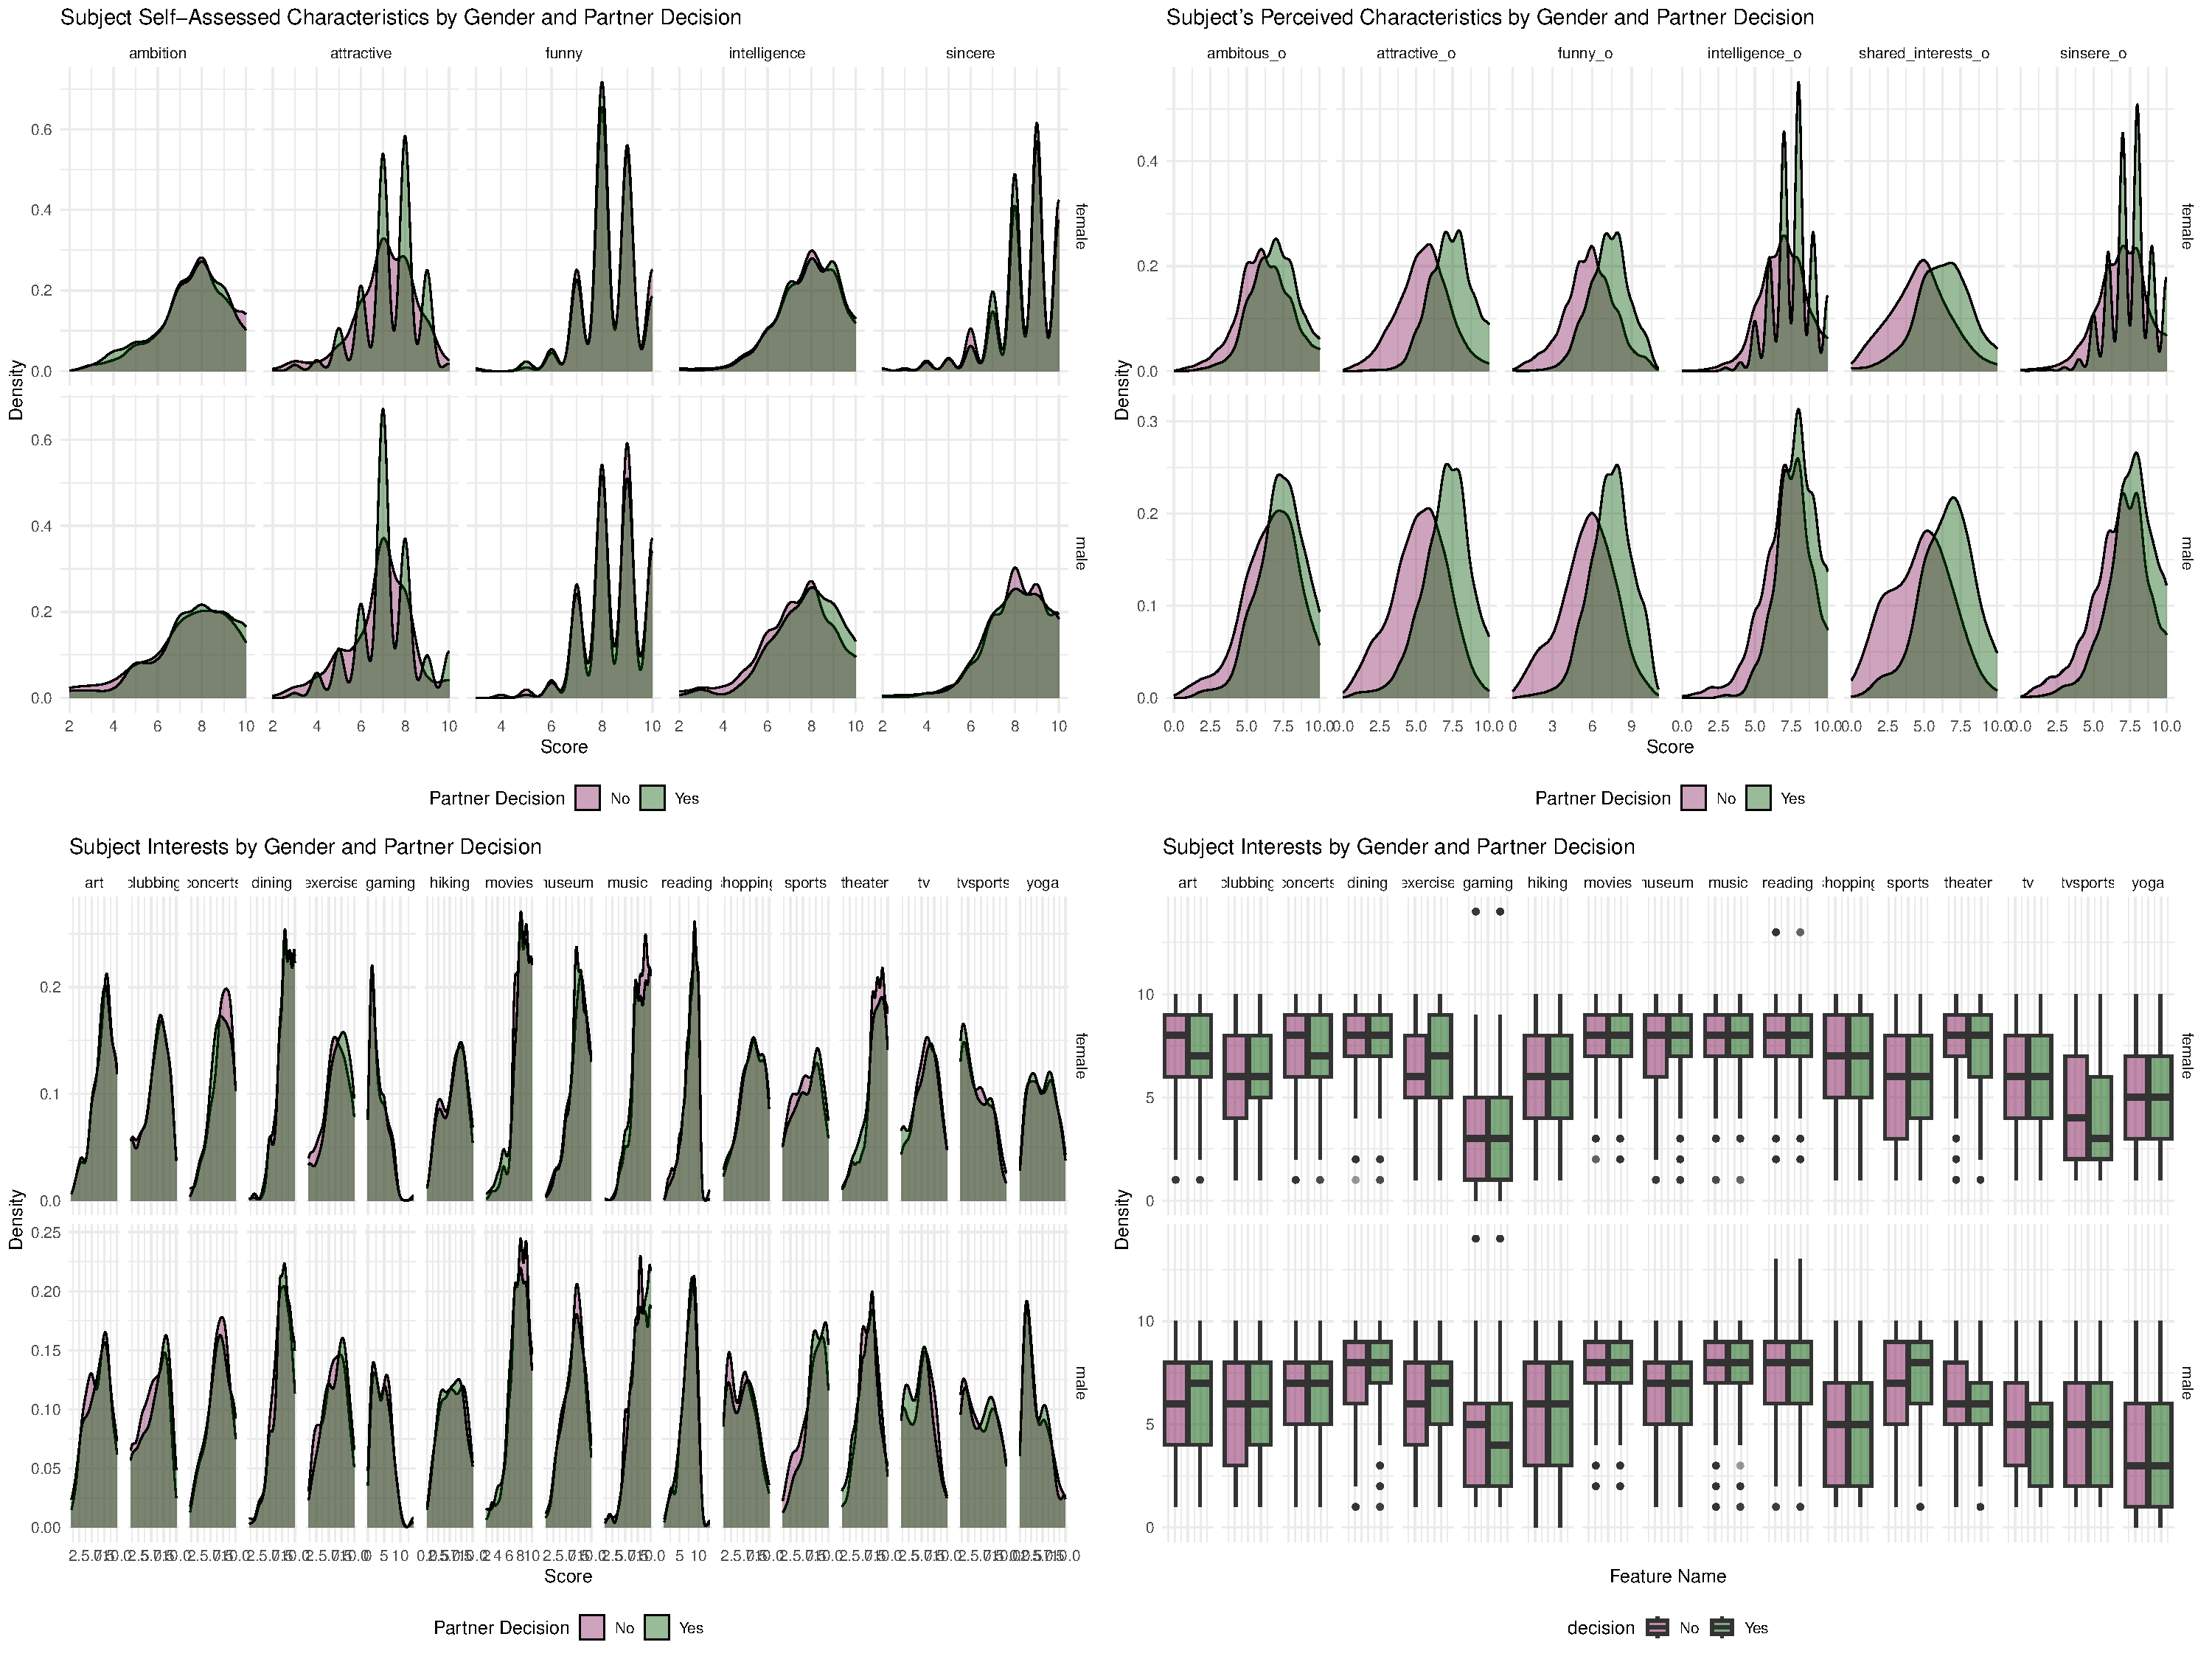
\includegraphics[keepaspectratio]{EDA-Plan_files/figure-pdf/subject_char_gender-1.pdf}}

\begin{itemize}
\item
  \textbf{Gender and race interaction}:

  \begin{itemize}
  \tightlist
  \item
    Same-race pairings were more likely to result in ``yes'' decisions.
    Male subjects tended to receive more ``no'' responses overall.
  \item
    Male partners showed favourable bias towards female subjects of
    White or Latina backgrounds, while other groups faced lower
    acceptance.
  \item
    Female partners, appeared more race-conscious when evaluating male
    subjects, with Asian-American male subjects received a higher
    proportion of unfavourable responses.
  \end{itemize}

  \pandocbounded{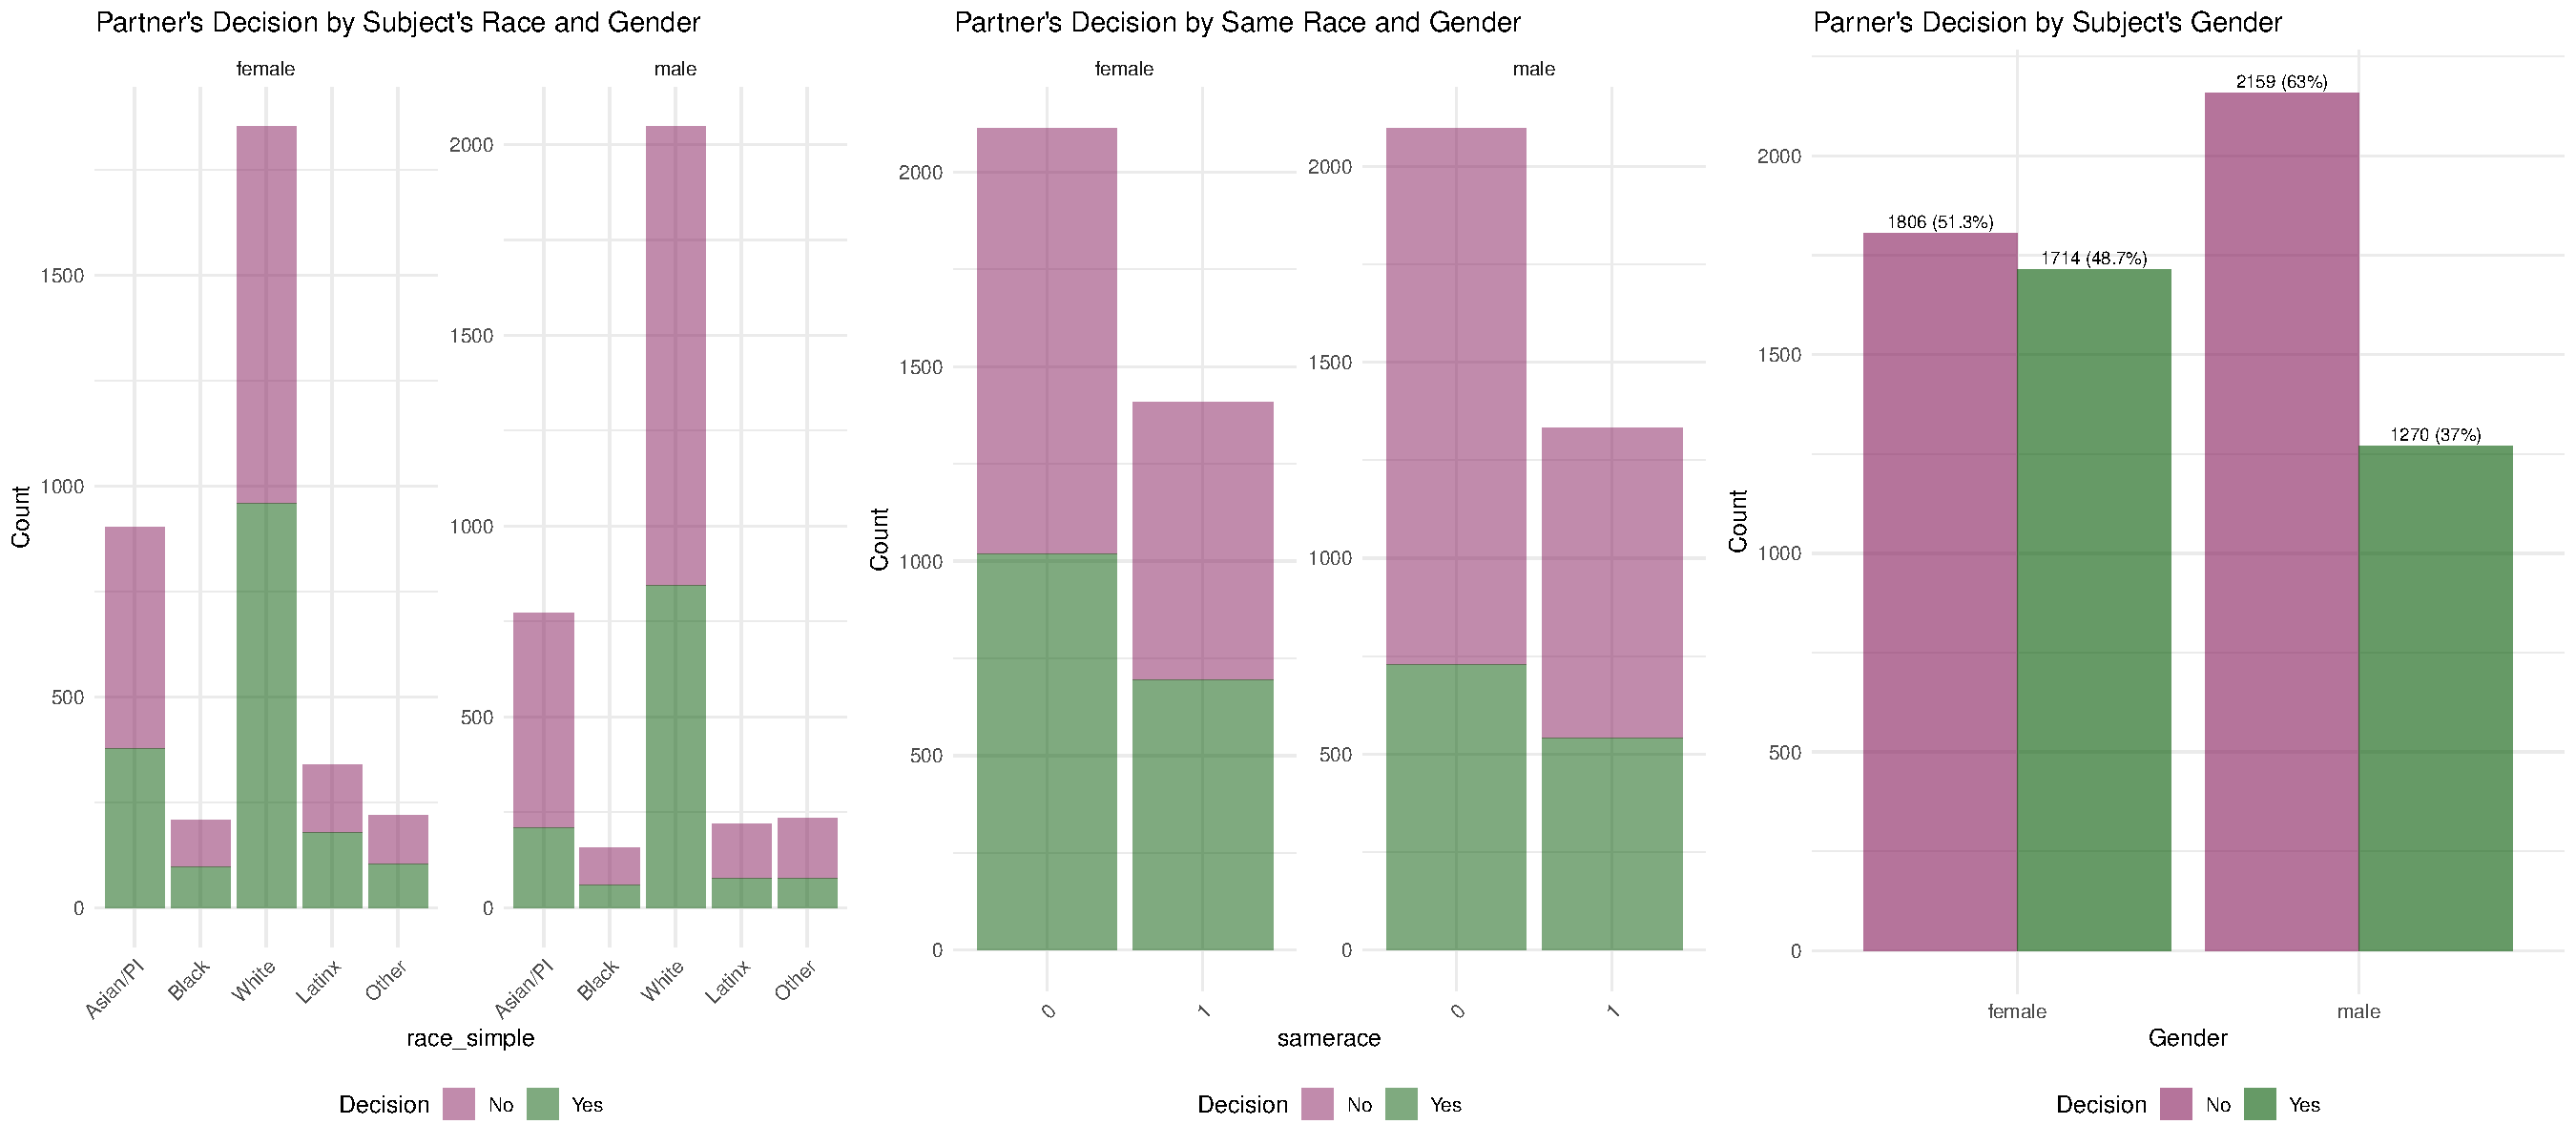
\includegraphics[keepaspectratio]{EDA-Plan_files/figure-pdf/gender_-1.pdf}}
\end{itemize}

\subsubsection{Outliers}\label{outliers}

Boxplots reveal several potential outliers beyond the interquartile
range, especially in self reported ratings (1-10 scales with values
outside the range).

\begin{itemize}
\item
  Models sensitive to outliers (e.g., Logistic Regression, LDA) may be
  adversely affected.
\item
  Tree based models and ensemble methods are more robust to outliers and
  will be targeted as part of the project.
\end{itemize}

\pandocbounded{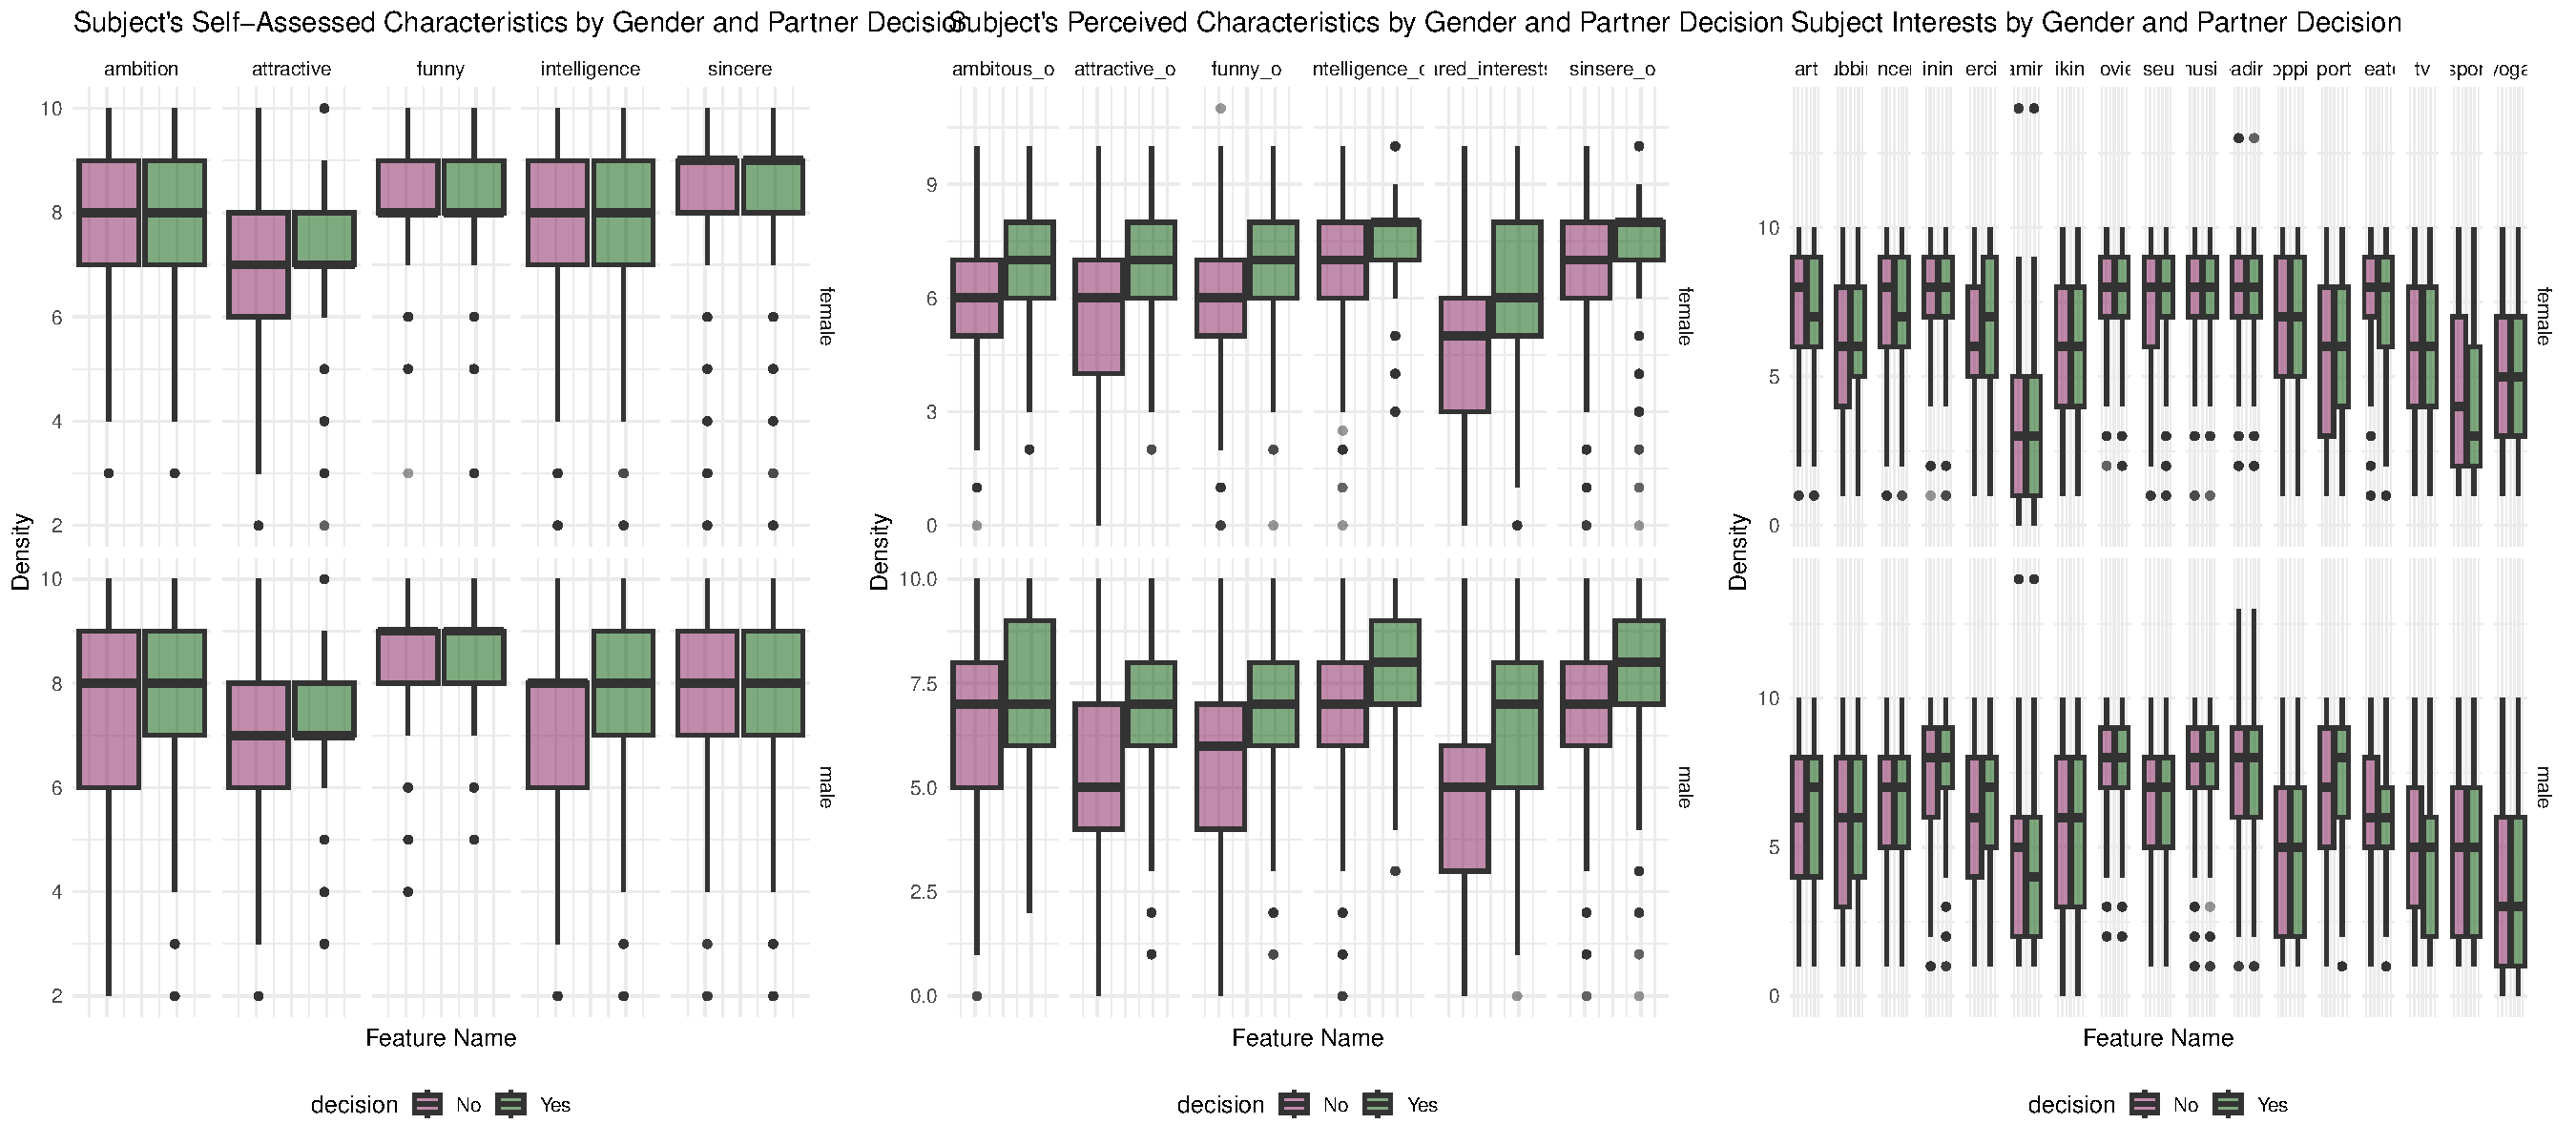
\includegraphics[keepaspectratio]{EDA-Plan_files/figure-pdf/outliers-1.pdf}}

\subsubsection{Normality}\label{normality}

The assumption of multivariate normality is violated. Predictors show
high skewness, heavy tails, and multimodality. These characteristics
limit the applicability of parametric models such as LDA, and favour
non-parametric models such as tree based and ensemble methods, kNN and
SVM may better capture nonlinear relationships, though kNN is sensitive
to high dimensionality.

\subsection{Classification Implementation
Plan}\label{classification-implementation-plan}

We have completed data cleaning \& wrangling, as well as EDA.

Next steps are as follows.

(show in visual: For high dimensional data, can you plot the data in a
lower dimension for visualization purpose (e.g.~PCA plots))

\subsubsection{Evaluation Metrics}\label{evaluation-metrics}

Given the balanced dataset, \textbf{accuracy} will serve as our primary
metric. However, to better capture nuances, we will also consider:

\begin{itemize}
\tightlist
\item
  \textbf{Log Loss}: Penalizes confident but incorrect predictions.
\item
  \textbf{ROC-AUC}: Evaluates overall discriminatory ability across
  thresholds.
\end{itemize}

\subsubsection{Modelling Approach}\label{modelling-approach}

Based on the EDA, we will perform the following models in order of
suitability:

\begin{itemize}
\tightlist
\item
  \textbf{Random forest:} easy to interpret, and tune to prevent
  overfitting. This will be highly regarded as
\item
  \textbf{Trees}: easy to interpret but prone to overfitting, which
  would mean that we would need to include hyperparameter tuning to
  reduce overfitting.
\item
  \textbf{Logistic Regression}: May remain effective given the large
  sample size, despite assumption violations.
\item
  \textbf{LDA}: Likely underperform due to non-normality and outliers.
\item
  \textbf{kNN \& SVM}: Better suited for non-linear boundaries but
  challenged by class overlap and dimensionality. kNN is also
  computationally expensive for large datasets (must compute distance to
  all training points) and is sensitive to high dimensions and
  irrelevant features. Sensitive to feature scaling (distance-based). No
  model coefficients or interpretability which will has lowered this in
  terms of suitability as we're hoping to interpret features relations
  to gain insights from the model.
\item
  \textbf{Boosting}: sequentially corrects errors; XGBoost adds
  regularisation.
\item
  We will Compare models, SHAP values/feature importances for
  interpretation.
\end{itemize}

\subsection{Appendix}\label{appendix}

\subsubsection{Feature Names}\label{feature-names}

\begin{table}
\fontsize{12.0pt}{14.4pt}\selectfont
\begin{tabular*}{\linewidth}{@{\extracolsep{\fill}}ccc}
\toprule
Variable.Group & Variable.Name & Variable.Description \\ 
\midrule\addlinespace[2.5pt]
Self reported Subject & gender & Gender of self \\ 
Self reported Subject & d\_age & Difference in age \\ 
Self reported Subject & race & Race of self \\ 
Self reported Subject & samerace & Whether the two persons have the same race or not. \\ 
Partner: Preferences Ratings & race\_o & Race of partner \\ 
Partner: Preferences Ratings & attractive\_o & Rating by partner (about me) at night of event on attractiveness \\ 
Partner: Preferences Ratings & sincere\_o & Rating by partner (about me) at night of event on sincerity \\ 
Partner: Preferences Ratings & intelligence\_o & Rating by partner (about me) at night of event on intelligence \\ 
Partner: Preferences Ratings & funny\_o & Rating by partner (about me) at night of event on being funny \\ 
Partner: Preferences Ratings & ambitous\_o & Rating by partner (about me) at night of event on being ambitious \\ 
Partner: Preferences Ratings & shared\_interests\_o & Rating by partner (about me) at night of event on shared interest \\ 
Subject Self: Self-evaluation & attractive & Rate yourself - attractiveness \\ 
Subject Self: Self-evaluation & sincere & Rate yourself - sincerity \\ 
Subject Self: Self-evaluation & intelligence & Rate yourself - intelligence \\ 
Subject Self: Self-evaluation & funny & Rate yourself - being funny \\ 
Subject Self: Self-evaluation & ambition & Rate yourself - ambition \\ 
Subject Self: Degree of Interest on common Interests & sports & Your own interests [1-10] \\ 
Subject Self: Degree of Interest on common Interests & tvsports & Your own interests [1-10] \\ 
Subject Self: Degree of Interest on common Interests & exercise & Your own interests [1-10] \\ 
Subject Self: Degree of Interest on common Interests & dining & Your own interests [1-10] \\ 
Subject Self: Degree of Interest on common Interests & museums & Your own interests [1-10] \\ 
Subject Self: Degree of Interest on common Interests & art & Your own interests [1-10] \\ 
Subject Self: Degree of Interest on common Interests & hiking & Your own interests [1-10] \\ 
Subject Self: Degree of Interest on common Interests & gaming & Your own interests [1-10] \\ 
Subject Self: Degree of Interest on common Interests & clubbing & Your own interests [1-10] \\ 
Subject Self: Degree of Interest on common Interests & reading & Your own interests [1-10] \\ 
Subject Self: Degree of Interest on common Interests & tv & Your own interests [1-10] \\ 
Subject Self: Degree of Interest on common Interests & theater & Your own interests [1-10] \\ 
Subject Self: Degree of Interest on common Interests & movies & Your own interests [1-10] \\ 
Subject Self: Degree of Interest on common Interests & concerts & Your own interests [1-10] \\ 
Subject Self: Degree of Interest on common Interests & music & Your own interests [1-10] \\ 
Subject Self: Degree of Interest on common Interests & shopping & Your own interests [1-10] \\ 
Subject Self: Degree of Interest on common Interests & yoga & Your own interests [1-10] \\ 
Results & decision\_o & Decision of partner at night of event. \\ 
\bottomrule
\end{tabular*}
\end{table}

\subsection{References}\label{references}

\begin{itemize}
\item
  Fisman, R., Iyengar, S. S., Kamenica, E., \& Simonson, I. (2006).
  Gender differences in mate selection: Evidence from a speed dating
  experiment. \emph{The Quarterly Journal of Economics, 121}(2),
  673--697. \url{https://doi.org/10.1162/qjec.2006.121.2.673}
\item
  OpenML. (n.d.). \emph{Speed Dating Dataset (ID 40536)}. Retrieved
  August 30, 2025, from
  \url{https://www.openml.org/search?type=data&sort=version&status=any&order=asc&exact_name=SpeedDating&id=40536}
\end{itemize}




\end{document}
